\chapter{Mathematische Beweise}
Mathematik ist eine exakte Wissenschaft. Diese Exaktheit verdankt die Mathematik der
Tatsache, dass Behauptungen \emph{bewiesen} werden k\"{o}nnen.  Der Begriff des \emph{Beweises} 
ist daher f\"{u}r die Mathematik zentral.  
In diesem Abschnitt gehen wir auf den mathematischen Beweisbegriff ein.  Wir beleuchten dabei nur die
praktische Seite und stellen verschiedene Methoden des Beweisens vor.  F\"{u}r eine theoretische Analyse des
Beweis-Begriffs ist die \emph{mathematische Logik} zust\"{a}ndig, die ein Teil der Informatik-Vorlesung ist.
Wir wenden uns hier den praktischen Beweis-Verfahren zu.
Grob k\"{o}nnen wir zwischen vier Arten von Beweisen unterscheiden:
\begin{enumerate}
\item direkten Beweisen,
\item indirekten Beweisen,
\item Beweise durch Fallunterscheidung, 
\item Beweise durch vollst\"{a}ndige Induktion.
\end{enumerate}

\section{Direkte Beweise}
Direkte Beweise sind die Beweise, die Sie bereits aus der Schule kennen.  Das wesentliche Hilfsmittel eines direkten Beweises
sind algebraische Umformungen.  Wir geben ein einfaches Beispiel f\"{u}r einen
direkten Beweis, ben\"{o}tigen daf\"{u}r aber zun\"{a}chst noch eine Definition.


\begin{Definition}[Pythagoreische Tripel] \hspace*{\fill} \\
Ein Tripel $\langle x, y, z \rangle \in \mathbb{N}\!\times\!\mathbb{N}\!\times\!\mathbb{N}$ hei\3t
\emph{Pythagoreisches Tripel}, falls
\\[0.2cm]
\hspace*{1.3cm}
$x^2 + y^2 = z^2$
\\[0.2cm]
gilt.  In diesem Fall sind die Zahlen $x$, $y$ und $z$ nach dem Satz des Pythagoras die L\"{a}ngen eines
rechtwinkligen Dreiecks:  $x$ und $y$ sind die L\"{a}ngen der Katheten, w\"{a}hrend $z$ die L\"{a}nge der Hypothenuse
ist.
\end{Definition}

\example
Das Tripel $\langle 3, 4, 5 \rangle$ ist ein pythagoreisches Tripel, denn es gilt
\\[0.2cm]
\hspace*{1.3cm}
$3^2 + 4^2 = 9 + 16 = 25 = 5^2$. \eox


\begin{Satz} 
Es seien $u$ und $v$ nat\"{u}rliche Zahlen mit $u > v$.  Dann ist
\\[0.2cm]
\hspace*{1.3cm}
$\bigl\langle u^2 - v^2,\; 2 \cdot u \cdot v,\; u^2 + v^2 \bigr\rangle$
\\[0.2cm]
ein pythagoreisches Tripel.  
\end{Satz}

\proof
Wir m\"{u}ssen zeigen, dass
\begin{equation}
  \label{eq:pyth}
\bigl( u^2 - v^2 \bigr)^2 + \bigl(2 \cdot u \cdot v \bigr)^2 = \bigl(u^2 + v^2\bigr)^2  
\end{equation}
gilt.  Dazu vereinfachen wir die beiden Seiten dieser Gleichung auf algebraischem Wege.
Wir benutzen dabei lediglich die beiden binomischen Formeln 
$(a + b)^2 = a^2 + 2 \cdot a \cdot b + b^2$ und
$(a - b)^2 = a^2 - 2 \cdot a \cdot b + b^2$.
Die Rechnung verl\"{a}uft wie folgt:
\\[0.2cm]
\hspace*{1.3cm}
$
\begin{array}[t]{cl}
   & \bigl( u^2 - v^2 \bigr)^2 + \bigl(2 \cdot u \cdot v \bigr)^2 \\[0.2cm]
 = & u^4 - 2 \cdot u^2 \cdot v^2 + v^4  + 4 \cdot u^2 \cdot v^2 \\[0.2cm]
 = & u^4 + 2 \cdot u^2 \cdot v^2 + v^4 \\[0.2cm]
 = & \bigl(u^2 + v^2\bigr)^2 
\end{array}
$
\\[0.2cm]
Damit haben wir die linke Seite der Gleichung (\ref{eq:pyth}) in die rechte Seite umgeformt. \qed

Als ein weiteres Beispiel f\"{u}r einen direkten Beweis betrachten wir das folgende Logarithmen-Gesetz.

\begin{Satz}
  Es seien $a,b,c$ positive reelle Zahlen.  Dann gilt
  \\[0.2cm]
  \hspace*{1.3cm}
  $\ds\log_a(b) = \frac{\log_c(b)}{\log_c(a)}$.
\end{Satz}

\proof
Nach Definition des Logarithmus gilt
\\[0.2cm]
\hspace*{1.3cm}
$b = a^{\log_a(b)}$.
\\[0.2cm]
Nehmen  wir auf beiden Seiten dieser Gleichung den Logarithmus zur Basis $c$, erhalten wir die Gleichung
\\[0.2cm]
\hspace*{1.3cm}
$\log_c(b) = \log_c\bigl(a^{\log_a(b)}\bigr)$.
\\[0.2cm]
Auf Grund des Logarithmen-Gesetzes $\log_c(a^x) = x \cdot \log_c(a)$ ist diese Gleichung zu
der  Gleichung
\\[0.2cm]
\hspace*{1.3cm}
$\log_c(b) = \log_a(b) \cdot \log_c(a)$
\\[0.2cm]
\"{a}quivalent.  Teilen wir beide Seiten dieser Gleichung durch $\log_c(a)$, so erhalten wir die Gleichung
\\[0.2cm]
\hspace*{1.3cm}
$\ds\frac{\log_c(b)}{\log_c(a)} = \log_a(b)$
\\[0.2cm]
und haben damit die Behauptung bewiesen.
\qed

\remark
Der letzte Satz zeigt Ihnen, wie Sie den Logarithmus zu einer beliebigen Basis mit einem
Taschenrechner berechnen k\"{o}nnen, auf dem nur der nat\"{u}rliche Logarithmus fest verdrahtet ist, denn es gilt
\\[0.2cm]
\hspace*{1.3cm}
$\ds\log_a(b) = \frac{\ln(b)}{\ln(a)}$.
\eox


\section{Indirekte Beweise}
Wollen wir eine Aussage $A$ auf indirektem Wege nachweisen, so nehmen wir an, dass $A$
nicht gilt, wir nehmen also an, dass die Aussage $\neg A$ richtig ist.  Wir versuchen dann
weiter, aus dieser Annahme eine offensichtlich falsche Aussage herzuleiten, beispielsweise
die Aussage, dass $1 = 2$ gilt.  Wenn dies gelingt, dann k\"{o}nnen wir r\"{u}ckw\"{a}rts schlie\3en,
dass die Annahme $\neg A$ falsch sein muss und dass folglich die Aussage $A$ wahr ist.
Wir geben sp\"{a}ter einige Beispiele f\"{u}r indirekte Beweise.
\vspace*{0.2cm}

Bevor wir das erste Beispiel pr\"{a}sentieren k\"{o}nnen, wiederholen wir den Begriff der \emph{geraden} und
\emph{ungeraden} Zahlen.  Eine nat\"{u}rliche Zahl $n$ ist gerade, wenn Sie durch $2$ teilbar ist.  Eine
solche Zahl l\"{a}sst sich also immer in der Form $n = 2 \cdot k$ mit $k \in \mathbb{N}$ schreiben.
Eine nat\"{u}rliche Zahl $n$  ist ungerade, wenn sie nicht durch $2$ teilbar ist.  Eine ungerade Zahl
hat bei Division durch $2$ also den Rest $1$ und l\"{a}sst sich damit immer in der Form $2 \cdot k + 1$
darstellen, wobei $k \in \mathbb{N}_0$ ist.

\begin{Lemma} \label{lemma:b1}
  Es seien $p \in \mathbb{N}$ und das Quadrat $p^2$ sei eine gerade Zahl.
  Dann ist $p$ eine gerade Zahl.
\end{Lemma}

\proof
Wir f\"{u}hren den Beweis indirekt und nehmen an, dass $p$ ungerade ist.  Damit l\"{a}sst sich $p$  in der Form
\\[0.2cm]
\hspace*{1.3cm}
$p = 2 \cdot q + 1$ \quad mit \quad $q \in \mathbb{N}_0$
\\[0.2cm]
schreiben.  Bilden wir das Produkt $p^2 = p \cdot p$, so finden wir
\\[0.2cm]
\hspace*{1.3cm}
$
\begin{array}[t]{rcl}
  p \cdot p & = & (2 \cdot q + 1) \cdot (2 \cdot q + 1) \\[0.1cm]
            & = & 4 \cdot q^2 + 4 \cdot q + 1           \\[0.1cm]
            & = & 2 \cdot (2 \cdot q^2 + 2 \cdot q) + 1 
\end{array}
$
\\[0.2cm]
Da die Zahl $2 \cdot (2 \cdot q^2 + 2 \cdot q) + 1$ die Form $2 \cdot s + 1$ mit
$s = (2 \cdot q^2 + 2 \cdot q)$ hat, handelt es sich um eine ungerade Zahl.
Diese Zahl ist aber gleich $p^2$ und damit haben wir einen Widerspruch zur
Voraussetzung erhalten.  Dieser Widerspruch zeigt, dass die Annahme, dass $p$ ungerade ist, falsch
sein muss.  Folglich ist $p$ gerade.
\qed

\begin{Satz}
  Die Quadratwurzel aus 2 ist irrational, es gilt $\sqrt{2} \not\in \mathbb{Q}$.
\end{Satz}

\proof
Wir f\"{u}hren den Beweis indirekt und machen die Annahme, dass $\sqrt{2} \in \mathbb{Q}$ ist.  Jede positive
rationale Zahl l\"{a}sst sich in der Form $\bruch{p}{q}$ mit $p,q \in \mathbb{N}$ schreiben.  Dabei k\"{o}nnen
wir zus\"{a}tzlich annehmen, dass  $p$ und $q$ keinen von 1 verschiedenen gemeinsamen Teiler haben, denn
wenn $p$ und $q$ einen gemeinsamen Teiler $r > 1$ h\"{a}tten, k\"{o}nnten wir durch $r$ k\"{u}rzen.  Nach unserer 
Annahme gilt also
\begin{equation}
  \label{eq:b1}
  \sqrt{2} = \bruch{p}{q} \quad \mbox{mit $\textsl{ggt}(p,q) = 1$}.
\end{equation}
Die Funktion $\textsl{ggt}(p,q)$ berechnet hier den gr\"{o}\3ten gemeinsamen Teiler von $p$ und $q$.   
Da $p$ und $q$ keinen echten gemeinsamen Teiler mehr haben, einen eventuellen gemeinsamen Teiler
haben wir ja gek\"{u}rzt, gilt $\textsl{ggt}(p, q) = 1$.  Quadrieren wir  Gleichung (\ref{eq:b1}), so
verschwindet die Quadratwurzel auf der linken Seite der Gleichung und wir erhalten die Gleichung
\begin{equation}
  \label{eq:b2}
  2 = \bruch{p^2}{q^2}.
\end{equation}
Diese Gleichung multiplizieren wir mit $q^2$.  Das ergibt
\begin{equation}
  \label{eq:b3}
  2 \cdot q^2 = p^2.
\end{equation}
Damit sehen wir, dass $2$ ein Teiler von $p^2$ ist.  Damit ist die Zahl $p^2 = p \cdot p$ also eine gerade Zahl.
Nach dem eben bewiesenen Lemma muss dann auch die Zahl $p$ gerade sein.
Also ist $2$ auch ein Teiler von $p$ und damit schreibt sich $p$ in der Form $p = 2 \cdot s$ mit $s
\in \mathbb{N}$.  Setzen 
wir die Gleichung $p = 2 \cdot s$ in Gleichung (\ref{eq:b3}) ein, so erhalten wir 
\begin{equation}
  \label{eq:b4}
  2 \cdot q^2 = (2 \cdot s)^2 = 4 \cdot s^2.
\end{equation}
Diese Gleichung teilen wir durch $2$ und haben
\begin{equation}
  \label{eq:b5}
  q^2 = (2 \cdot s)^2 = 2 \cdot s^2.
\end{equation}
Gleichung (\ref{eq:b5}) zeigt nun, dass $q^2$ eine gerade Zahl ist und wieder nach dem Lemma
\ref{lemma:b1} k\"{o}nnen wir folgern, dass auch  $q$ gerade ist.  Folglich ist $q$ durch $2$ teilbar.
Damit sind dann aber $p$ und $q$ nicht teilerfremd und wir haben einen Widerspruch zu der
Annahme, dass $\sqrt{2}$ sich als Bruch $\bruch{p}{q}$ zweier nat\"{u}rlicher Zahlen $p$ und $q$
darstellen l\"{a}sst, denn einen solchen Bruch k\"{o}nnen wir immer so k\"{u}rzen, dass $p$ und $q$ teilerfremd
sind. 
\qed


Ein anderes typisches Beispiel f\"{u}r einen indirekten Beweis ist der Nachweis der
Nicht-Abz\"{a}hlbarkeit der Potenz-Menge der nat\"{u}rlichen Zahlen.

\begin{Definition}[Abz\"{a}hlbar] \hspace*{\fill} \\
Eine unendliche Menge $M$ hei\3t \colorbox{yellow}{\emph{abz\"{a}hlbar}}, wenn eine 
\underline{sur}j\underline{ektive} Funktion
\\[0.2cm]
\hspace*{1.3cm}
$f: \mathbb{N} \rightarrow M$
\\[0.2cm]
existiert.  Dabei nennen wir eine Funktion $f:A \rightarrow B$  \emph{surjektiv} genau
dann, wenn es zu jedem $y \in B$ ein $x \in A$ gibt, so dass $f(x) = y$ ist:
\\[0.2cm]
\hspace*{1.3cm}
$\forall y \in B: \exists x \in A: f(x) = y$.  \eox
\end{Definition}

Die Idee bei dieser Definition ist, dass die Menge  $M$ in einem gewissen Sinne nicht mehr Elemente hat
als die Menge der nat\"{u}rlichen Zahlen, denn die Elemente k\"{o}nnen ja \"{u}ber die Funktion $f$
aufgez\"{a}hlt werden, wobei wir eventuelle Wiederholungen eines Elements zulassen wollen.

\example
Die Menge $\mathbb{Z}$ der ganzen Zahlen ist abz\"{a}hlbar, denn die Funktion
\\[0.2cm]
\hspace*{1.3cm}
$f: \mathbb{N} \rightarrow \mathbb{Z}$,
\\[0.2cm]
die durch die Fallunterscheidung
\\[0.2cm]
\hspace*{1.3cm}
$f(n) := \left\{ \begin{array}[c]{ll}
                 (n - 1) / 2 + 1  & \mbox{falls $n \modulo 2 = 1$}  \\[0.2cm]
                 - (n - 2) / 2          & \mbox{falls $n \modulo 2 = 0$}
                 \end{array}
         \right.
$ 
\\[0.2cm]
definiert ist, ist surjektiv.  Um dies einzusehen, zeigen wir zun\"{a}chst, dass $f$ wohldefiniert ist.
Dazu ist zu zeigen, dass $f(n)$ tats\"{a}chlich in jedem Fall eine ganze Zahl ist.
\begin{enumerate}
\item $n \modulo 2 = 1$:  Dann ist $n$ ungerade, also ist $(n-1)$ gerade und die Division
      $(n-1)/2$ liefert eine ganze Zahl.
\item $n \modulo 2 = 0$:  In diesem Fall ist $n$ gerade.  Damit ist auch $(n-2)$ gerade und daher
      liefert jetzt die Division $n/2$ eine ganze Zahl.
\end{enumerate}
Es bleibt zu zeigen, dass $f$ surjektiv ist.  Wir m\"{u}ssen also zeigen, dass es f\"{u}r jedes 
$z \in \mathbb{Z}$ eine nat\"{u}rliche Zahl $n$ gibt, so dass $f(n) = z$ ist.  Wir f\"{u}hren diesen Nachweis
mittels einer Fall-Unterscheidung:
\begin{enumerate}
\item Fall: $z > 0$.
  
      Wir definieren $n := 2 \cdot (z - 1) + 1$.  Wegen $z >0$ gilt $n > 0$ und damit ist $n$
      tats\"{a}chlich eine nat\"{u}rliche Zahl.  Au\3erdem ist klar, dass $n$ ungerade ist. Daher gilt
      \\[0.2cm]
      \hspace*{0.3cm}
      $f(n) = (n - 1)/2 + 1 = \bigl(\bigl(2 \cdot (z - 1) + 1\bigr) - 1\bigr)/2 + 1 
            = \bigl(2 \cdot (z - 1)/2\bigr) + 1= z-1 + 1 = z
      $.
      \\[0.2cm]
      Also gilt $f(n) = z$.
\item Fall: $z \leq 0$.

      Wir definieren $n := - 2 \cdot (z - 1)$.  Wegen $z \leq 0$ ist klar, dass $n$ eine gerade 
      nat\"{u}rliche Zahl ist.  Damit haben wir
      \\[0.2cm]
      \hspace*{1.3cm}
      $f(n) = -\bigl(-2 \cdot (z - 1) - 2\bigr)/2 = z$.
      \\[0.2cm]
      Also gilt ebenfalls $f(n) = z$.
\end{enumerate}
Damit ist die Sujektivit\"{a}t von $f$ gezeigt und somit ist $\mathbb{Z}$ abz\"{a}hlbar.
\qed

Den Beweis des letzten Satzes haben wir direkt gef\"{u}hrt, aber zum Nachweis des n\"{a}chsten Satzes werden wir
einen indirekten Beweis ben\"{o}tigen.  Vorab noch eine Definition.

\begin{Definition}[\"{U}berabz\"{a}hlbar] \lb
Eine unendliche Menge hei\3t \colorbox{yellow}{\emph{\"{u}berabz\"{a}hlbar}}, wenn sie \underline{nicht} abz\"{a}hlbar ist.
\end{Definition}

\begin{Satz}
  Die Potenzmenge der Menge der nat\"{u}rlichen Zahlen ist \"{u}berabz\"{a}hlbar.
\end{Satz}

\proof
Wir f\"{u}hren den Beweis indirekt und nehmen an, dass $2^{\mathbb{N}}$ abz\"{a}hlbar ist.  Dann gibt es also
eine Funktion
\\[0.2cm]
\hspace*{1.3cm}
$f: \mathbb{N} \rightarrow 2^{\mathbb{N}}$,
\\[0.2cm]
die surjektiv ist.  Wir definieren nun die Menge $C$ wie folgt:
\\[0.2cm]
\hspace*{1.3cm}
$C := \bigl\{ n \in \mathbb{N} \bigm| n \not\in f(n) \bigr\}$.
\\[0.2cm]
Offenbar ist $C$ eine Teilmenge der Menge der nat\"{u}rlichen Zahlen und damit gilt $C \in 2^{\mathbb{N}}$.
Da die Funktion $f$ nach unserer Annahme surjektiv ist, gibt es also eine nat\"{u}rliche Zahl $n_0$, so
dass 
\\[0.2cm]
\hspace*{1.3cm}
$C = f(n_0)$
\\[0.2cm]
gilt.  Wir untersuchen nun, ob $n_0 \in C$ gilt.  Dazu betrachten wir die folgende Kette von
\"{A}quivalenzen: 
\\[0.2cm]
\hspace*{1.3cm}
$
\begin{array}[t]{cl}
                & n_0 \in C                                                      \\[0.2cm]
\Leftrightarrow & n_0 \in \bigl\{ n \in \mathbb{N} \bigm| n \not\in f(n) \bigr\} \\[0.2cm]
\Leftrightarrow & n_0 \not\in f(n_0)                                             \\[0.2cm]
\Leftrightarrow & n_0 \not\in C                                               
\end{array}
$
\\[0.2cm]
Wir haben also
\\[0.2cm]
\hspace*{1.3cm}
$n_0 \in C \;\Leftrightarrow\; n_0 \not\in C \qquad \color{red}{\lightning}$
\\[0.2cm]
gezeigt und das ist ein offensichtlicher Widerspruch. \qed

\remark
Wir haben soeben gezeigt, dass es in gewisser Weise mehr Mengen von nat\"{u}rlichen Zahlen gibt, als es
nat\"{u}rliche Zahlen gibt.  In \"{a}hnlicher Weise kann gezeigt werden, dass die Menge $\mathbb{R}$ der reellen
Zahlen \"{u}berabz\"{a}hlbar ist.  

\exercise
Zeigen Sie, dass das Intervall
\\[0.2cm]
\hspace*{1.3cm}
$[0,1[ := \{ x \in \mathbb{R} \mid 0 \leq x \wedge x < 1 \}$ 
\\[0.2cm]
\"{u}berabz\"{a}hlbar ist.  Nehmen Sie dazu an, dass die Zahlen $x \in [0,1[$ in der Form
\\[0.2cm]
\hspace*{1.3cm}
$ x = 0, d_1 d_2 d_3 \cdots$ \quad mit $d_i \in \{ 0, \cdots, 9 \}$  f\"{u}r alle $i \in \mathbb{N}$
\\[0.2cm]
dargestellt sind, es gilt dann also
\\[0.2cm]
\hspace*{1.3cm}
$\ds x = \sum\limits_{i=1}^\infty d_i \cdot \Bigl(\frac{1}{10}\Bigr)^{i}$.
\\[0.2cm]
Um sicher zu stellen, dass diese Darstellung eindeutig ist, fordern wir, dass diese Darstellung
nicht auf ``Periode Neun'' endet, es d\"{u}rfen also ab einem bestimmten Index $n \in \mathbb{N}$ nicht
alle Ziffern $d_i$ den Wert $9$ haben:
\\[0.2cm]
\hspace*{1.3cm}
$\neg \exists n \in \mathbb{N}: \forall i \in \mathbb{N}: i \geq n \rightarrow c_i = 9$.
\\[0.2cm]
F\"{u}hren Sie den Beweis indirekt und nehmen Sie an, dass es eine surjektive Funktion 
\\[0.2cm]
\hspace*{1.3cm}
$f: \mathbb{N} \rightarrow [0,1[$
\\[0.2cm]
gibt, die die Menge $[0,1[$ aufz\"{a}hlt.  Dann gibt es auch eine Funktion
\\[0.2cm]
\hspace*{1.3cm}
$g: \mathbb{N} \times \mathbb{N} \rightarrow \{0, \cdots, 9\}$
\\[0.2cm]
so dass $g(n,i)$ die $i$-te Nachkommastelle von $f(n)$ berechnet:
\\[0.2cm]
\hspace*{1.3cm}
$f(n) = 0,g(n,1) g(n,2) g(n,3) \cdots$.
\\[0.2cm]
Konstruieren Sie nun mit Hilfe dieser Funktion $g$ eine Zahl $c \in [0,1[$ in der Form
\\[0.2cm]
\hspace*{1.3cm}
$c = 0,c_1c_2c_3 \cdots$
\\[0.2cm]
so, dass sich ein Widerspruch ergibt.  Orientieren Sie sich dabei an der Konstruktion der Menge $C$ im
Beweis der \"{u}berabz\"{a}hlbarkeit von $2^\mathbb{N}$.  \exend

\exercise
Zeigen Sie, dass die Menge
\\[0.2cm]
\hspace*{1.3cm}
$\mathbb{N}^\mathbb{N} := \{ f \mid f: \mathbb{N} \rightarrow \mathbb{N} \}$,
\\[0.2cm]
also die Menge aller Funktionen von $\mathbb{N}$ nach $\mathbb{N}$ \"{u}berabz\"{a}hlbar ist.
\exend

\exercise
Zeigen Sie, dass die Menge $\mathbb{Q}_+$ der positiven rationalen Zahlen abz\"{a}hlbar ist.
\exend

\section{Beweise durch Fallunterscheidung}
Wir haben in dem Kapitel \"{u}ber Mengenlehre bereits eine ganze Reihe direkter Beweise gesehen.
Dort war es oft notwendig, den Beweis in zwei Teile aufzuspalten.
Um beispielsweise die Gleichheit zweier Mengen $A$ und $B$ zu zeigen, sind wir 
h\"{a}ufig so vorgegangen, dass wir zun\"{a}chst 
$A \subseteq B$ und anschlie\3end $B \subseteq A$ gezeigt haben.  So hatten wir beispielsweise  im
letzten Kapitel nachgewiesen, dass f\"{u}r eine \"{A}quivalenz-Relation $R$ aus der Beziehung $\pair(x,y) \in R$ die
Gleichung $[x]_R = [y]_R$ gefolgert werden kann.  Beim Beweis durch \emph{Fallunterscheidung} teilen
wir den Beweis ebenfalls in mehrere Teile auf.  Wir illustrieren das Konzept an einem Beispiel.

\begin{Satz}
  Es gibt irrationale Zahlen $x$ und $y$, so dass $x^y$ rational ist, es gilt also
  \\[0.2cm]
  \hspace*{1.3cm}
  $\exists x, y \in \mathbb{R}: x \not\in \mathbb{Q} \wedge y \not\in \mathbb{Q} \wedge x^y \in \mathbb{Q}$.
\end{Satz}

\proof
Im letzten Abschnitt haben wir bereits gezeigt, dass die Zahl $\sqrt{2}$ irrational ist.  Wir
betrachten nun die Zahl 
\\[0.2cm]
\hspace*{1.3cm}
$\sqrt{2}^{\sqrt{2}}$.
\\[0.2cm]
Es gibt nur zwei M\"{o}glichkeiten: Entweder ist die Zahl $\sqrt{2}^{\sqrt{2}}$ rational oder nicht.  Wir
untersuchen diese beiden F\"{a}lle getrennt.
\begin{enumerate}
\item Fall: $\sqrt{2}^{\sqrt{2}} \in \mathbb{Q}$.

      In diesem Fall definieren wir
      \\[0.2cm]
      \hspace*{1.3cm}
      $x := \sqrt{2}$ \quad und \quad $y := \sqrt{2}$.  
      \\[0.2cm]
      Da wir bereits wissen,
      dass $\sqrt{2} \not\in \mathbb{Q}$ ist, und da nach der Voraussetzung der
      Fallunterscheidung $x^y \in \mathbb{Q}$ gilt, haben wir in diesem Fall bereits Zahlen $x$ und
      $y$ mit der behaupteten Eigenschaft gefunden.
\item Fall:  $\sqrt{2}^{\sqrt{2}} \not\in \mathbb{Q}$.

      In diesem Fall definieren wir 
      \\[0.2cm]
      \hspace*{1.3cm}
      $x := \sqrt{2}^{\sqrt{2}}$ \quad und \quad $y := \sqrt{2}$.
      \\[0.2cm]
      Jetzt ist $x$ nach der Voraussetzung der Fallunterscheidung irrational und dass $y$ irrational
      ist, haben wir bereits fr\"{u}her bewiesen.  Au\3erdem gilt
      \\[0.2cm]
      \hspace*{1.3cm}
      $\ds x^y = \bigl(\sqrt{2}^{\sqrt{2}}\bigr)^{\sqrt{2}} = \sqrt{2}^{(\sqrt{2} \cdot \sqrt{2})} = \sqrt{2}^{2} = 2 \in \mathbb{Q}$,
      \\[0.2cm]
      so dass die Behauptung auch im zweiten Fall bewiesen ist.  \qed
\end{enumerate}

Beachten Sie, dass es uns bei dem letzten Beweis nicht m\"{o}glich war, die Zahlen $x$ und $y$ konkret
anzugeben.  Wir wissen nur, dass entweder die beiden Zahlen
\\[0.2cm]
\hspace*{1.3cm}
$x_1 := \sqrt{2}$ und $y_1 := \sqrt{2}$ \quad oder \quad die Zahlen $x_2 := \sqrt{2}^{\sqrt{2}}$ und $y_2 := \sqrt{2}$.
\\[0.2cm]
die behauptete Eigenschaft 
\\[0.2cm]
\hspace*{1.3cm}
$x \not\in \mathbb{Q} \wedge y \not\in \mathbb{Q} \wedge x^y \in \mathbb{Q}$
\\[0.2cm]
haben, aber der obige Beweis sagt nichts dar\"{u}ber, welches der beiden Paare $\pair(x_1,y_1)$ und
$\pair(x_2,y_2)$ tats\"{a}chlich die obige Eigenschaft hat.  Das war f\"{u}r den gerade angegebenen Beweis
auch nicht erforderlich: Wir haben nur gezeigt, dass es ein Paar $\pair(x,y)$ mit der Eigenschaft
\\[0.2cm]
\hspace*{1.3cm}
$x \not\in \mathbb{Q} \wedge y \not\in \mathbb{Q} \wedge x^y \in \mathbb{Q}$
\\[0.2cm]
geben muss, aber wir waren nicht in der Lage, $x$ und $y$ konkret auszurechnen.  Daher ist der obige
Beweis kein \emph{konstruktiver} Beweis:  Zwar zeigt der Beweis die Existenz eines Paares
$\pair(x,y)$ mit den gew\"{u}nschten Eigenschaften, aber das Paar $\pair(x,y)$ kann nicht konkret
angegeben werden.

\remark
Aus dem \href{http://en.wikipedia.org/wiki/Gelfond%27s_theorem}{Gelfond-Schneider-Theorem}
kann gefolgert werden, dass $\sqrt{2}^{\sqrt{2}} \not\in \mathbb{Q}$ gilt.  Der Nachweis dieses
Theorem liegt aufgrund seiner Tiefe deutlich au\3erhalb des Rahmens einer einf\"{u}hrenden Mathematik-Vorlesung.

\exercise
Zeigen Sie, dass f\"{u}r alle $n \in \mathbb{N}$ die Zahl
\\[0.2cm]
\hspace*{1.3cm}
$5 \cdot n^3 + 10 \cdot n$
\\[0.2cm]
stets durch $3$ teilbar ist.  \exend

% 5 * n * (n^2 + 2)
%
% n = 3 * k + 1
% n^2 + 2 = 9 * k + 6 * k + 1 + 2
%
% n = 3 * k + 2
% n^2 + 2 = 9 * k + 6 * k + 4 + 2

\section{Induktions-Beweise}
Die wichtigste Beweismethode in der Informatik ist der Beweis durch vollst\"{a}ndige Induktion. 
Die Induktion ist in der Informatik deshalb so wichtig, weil Sie zum Beweis der Korrektheit
rekursiver Funktionen ben�tigt wird.  Es sei
$F(n)$ eine Formel, in der die Variable $n$ vorkommt.  Um eine Aussage der Form
\\[0.2cm]
\hspace*{1.3cm}
$\forall n \in \mathbb{N}: F(n)$
\\[0.2cm]
zu beweisen, k\"{o}nnen wir wie folgt vorgehen.
\begin{enumerate}
\item Zun\"{a}chst zeigen wir, dass die Aussage f\"{u}r $n=1$ richtig ist, wir weisen also die G\"{u}ltigkeit der
      Formel $F(1)$ nach.

      Dieser Schritt wird als \emph{Induktions-Anfang} bezeichnet.
\item Dann zeigen wir, dass die Formel
      \\[0.2cm]
      \hspace*{1.3cm}
      $\forall n \in \mathbb{N} : \bigl( F(n) \rightarrow F(n+1)\bigr)$
      \\[0.2cm]
      gilt, wir zeigen also, dass jedesmal, wenn $F(n)$ gilt, auch $F(n+1)$ richtig sein muss.

      Dieser Schritt wird als \emph{Induktions-Schritt} bezeichnet.
\end{enumerate}
Insgesamt k\"{o}nnen wir dann schlie\3en, dass die Formel $F(n)$ f\"{u}r alle nat\"{u}rlichen Zahlen gilt, denn
zun\"{a}chst wissen wir, dass $F(1)$ gilt, nach dem Induktions-Schritt gilt dann auch $F(2)$, daraus folgt
dass auch $F(3)$ gilt, woraus wir auf die G\"{u}ltigkeit von $F(4)$ schlie\3en k\"{o}nnen.  Durch Fortf\"{u}hrung
dieser Argumentation schlie\3en wir insgesamt, dass $F(n)$ f\"{u}r jede beliebige Zahl richtig ist.  Diese
Argumentation ist zun\"{a}chst informal. Ein Beweis folgt.

\begin{Satz}
  Es sei $F(x)$ eine Formel. Dann gilt
  \\[0.2cm]
  \hspace*{1.3cm}
  $F(1) \wedge \forall n \in \mathbb{N}:\bigl(F(n) \rightarrow F(n+1)\bigr) \rightarrow 
   \forall n \in \mathbb{N}: F(n)
  $.
\end{Satz}

\proof
Wir nehmen an, dass
\\[0.2cm]
\hspace*{1.3cm}
$F(1) \wedge \forall n \in \mathbb{N}:\bigl(F(n) \rightarrow F(n+1)\bigr)$
\\[0.2cm]
richtig ist und zeigen, dass dann
\\[0.2cm]
\hspace*{1.3cm}
$\forall n \in \mathbb{N}:F(n)$
\\[0.2cm]
gilt.  Den Nachweis dieser Behauptung f\"{u}hren wir indirekt und nehmen an, dass
\\[0.2cm]
\hspace*{1.3cm}
$\neg\bigl(\forall n \in \mathbb{N}:F(n)\bigr)$
\\[0.2cm]
gilt.  Das ist aber \"{a}quivalent zu der Formel
\\[0.2cm]
\hspace*{1.3cm}
$\exists n \in \mathbb{N}:\neg F(n)$.
\\[0.2cm]
Wir definieren eine Menge $M$ als die Menge aller der Zahlen, f\"{u}r die $F(n)$ falsch ist:
\\[0.2cm]
\hspace*{1.3cm}
$M := \bigl\{ n \in \mathbb{N} \bigm| \neg F(n) \bigr\}$.
\\[0.2cm]
Nach unserer Annahme ist $M$ nicht leer.  Als Menge von nat�rlichen Zahlen muss  $M$ dann aber ein
kleinstes Element haben.  Wir definieren $n_0$ als das Minimum von $M$.
\\[0.2cm]
\hspace*{1.3cm}
$n_0 := \min( M) = \min\bigl(\bigl\{ n \in \mathbb{N} \bigm| \neg F(n) \bigr\}\bigr)$.
\\[0.2cm]
Also haben wir $\neg F(n_0)$ und wissen au\3erdem, dass f\"{u}r alle $n < n_0$ die Formel $F(n)$ gilt, denn
sonst w\"{a}re $n_0$ ja nicht das Minimum der Menge $M$.

Weiter schlie\3en wir dann aus der Tatsache, dass $F(1)$ gilt, dass $n_0 \not= 1$ ist.  
Aus $n_0 -1 < n_0$ folgt nun, dass $n_0-1 \not\in M$ ist, denn $n_0$ ist ja das Minimum von $M$.
Aus  $n_0-1 \not\in M$ folgt nach Definition von $M$, dass die Formel
\\[0.2cm]
\hspace*{1.3cm}
$F(n_0 - 1)$
\\[0.2cm]
gilt.  Aus der Formel $\forall n \in \mathbb{N}:\bigl( F(n) \rightarrow F(n+1)\bigr)$ k\"{o}nnen wir dann folgern, dass
\\[0.2cm]
\hspace*{1.3cm}
$F\bigl((n_0-1) +1\bigr)$
\\[0.2cm] 
gilt.  Also gilt $F(n_0)$ und das ist ein Widerspruch zur Definition von $n_0$. \qed

Wir geben nun einige typische Beispiele f\"{u}r Induktions-Beweise.  Die in diesen S\"{a}tzen behaupteten
Summenformeln sollten Sie sich gut merken, denn diese Formeln werden sp\"{a}ter bei der Analyse der Komplexit\"{a}t
von Algorithmen h\"{a}ufig verwendet.

\begin{Satz} Es gilt 
\\[0.2cm]
\hspace*{1.3cm}
$\ds\sum\limits_{i=1}^n i = \frac{1}{2} \cdot n \cdot (n+1)$ \quad f\"{u}r alle $n \in \mathbb{N}$.
\end{Satz}

\proof
Wir f\"{u}hren den Beweis durch Induktion nach $n$.
\begin{enumerate}
\item Induktions-Anfang: $n=1$.

      Wir haben einerseits
      \\[0.2cm]
      \hspace*{1.3cm}
      $\ds\sum\limits_{i=1}^1 i = 1$
      \\[0.2cm]
      und andererseits gilt auch
      \\[0.2cm]
      \hspace*{1.3cm}
      $\ds\frac{1}{2} \cdot 1 \cdot (1+1) = 1$.
      \\[0.2cm]
      Damit ist die Behauptung f\"{u}r $n=1$ richtig.
\item Induktions-Schritt: $n \mapsto n+1$.

      Wir k\"{o}nnen nun voraussetzen, dass
      \\[0.2cm]
      \hspace*{1.3cm}
      $\ds\sum\limits_{i=1}^n i = \frac{1}{2} \cdot n \cdot (n+1)$
      \\[0.2cm]
      f\"{u}r ein gegebenes festes $n$ gilt.  Diese Voraussetzung wird als \emph{Induktions-Voraussetzung}
      bezeichnet.  Wir m\"{u}ssen dann nachweisen, dass  die Behauptung auch
      f\"{u}r $n+1$ gilt, zu zeigen ist also 
      \\[0.2cm]
      \hspace*{1.3cm}
      $\ds\sum\limits_{i=1}^{n+1} i = \frac{1}{2} \cdot (n+1) \cdot \bigl((n+1)+1\bigr)$.
      \\[0.2cm]
      Wir formen beide Seiten dieser Gleichung getrennt um und beginnen mit der linken Seite.
      \\[0.2cm]
      \hspace*{1.3cm}
      $
      \begin{array}[t]{cll}
        &\ds \sum\limits_{i=1}^{n+1} i                                                       \\[0.5cm]
      = &\ds \sum\limits_{i=1}^{n} i + (n+1)          & \mbox{nach Definition der Summe}     \\[0.5cm]
      = &\ds \frac{1}{2} \cdot n \cdot (n+1) + (n+1)  & \mbox{nach Induktions-Voraussetzung} \\[0.3cm]
      = &\ds \frac{1}{2} \cdot \bigl( n^2 + n  + 2 \cdot(n+1)\bigr)  & \mbox{Hauptnenner} \\[0.3cm]
      = &\ds \frac{1}{2} \cdot \bigl( n^2 + 3 \cdot n  + 2 \bigr)  
      \end{array}
      $
      \\[0.2cm]
      Nun formen wir die rechte Seite um:
      \\[0.2cm]
      \hspace*{1.3cm}
      $
      \begin{array}[t]{cl}
         &\ds \frac{1}{2} \cdot (n+1) \cdot \bigl((n+1)+1\bigr) \\[0.3cm]
       = &\ds \frac{1}{2} \cdot (n+1) \cdot (n+2)               \\[0.3cm]
       = & \ds \frac{1}{2} \cdot (n^2  + 2 \cdot n + n + 2)     \\[0.3cm]
       = &\ds \frac{1}{2} \cdot (n^2  + 3 \cdot n + 2)  
      \end{array}
      $
      \\[0.2cm]
      Da beide Seiten identisch sind, ist der Beweis erbracht. \qed
\end{enumerate}


\exercise
Zeigen Sie, dass
\\[0.2cm]
\hspace*{1.3cm}
$\ds\sum\limits_{i=1}^{n} i^2 = \frac{1}{6} \cdot n \cdot (n+1) \cdot (2 \cdot n + 1)$ \quad
f\"{u}r alle $n \in \mathbb{N}$ 
\\[0.2cm]
gilt.  \exend

\exercise
Zeigen Sie, dass im Falle $q \not= 1$
\\[0.2cm]
\hspace*{1.3cm}
$\ds\sum\limits_{i=0}^{n} q^i = \bruch{q^{n+1} - 1}{q - 1}$ \quad
f\"{u}r alle $n \in \mathbb{N}_0$ 
\\[0.2cm]
gilt.  Wie lautet die Formel im Falle $q=1$? \exend


\begin{Satz}[M\"{a}chtigkeit der Potenz-Menge]
Es sei $M$ eine endliche Menge.  Dann gilt
\\[0.2cm]
\hspace*{1.3cm}
$\textsl{card}\bigl(2^M\bigr) = 2^{\textsl{card}(M)}$.
\end{Satz}

\proof
Es sei $n := \textsl{card}(M)$.  Dann hat $M$ die Form
\\[0.2cm]
\hspace*{1.3cm}
$M = \{ x_1, x_2, \cdots, x_n \}$.
\\[0.2cm]
Wir zeigen durch Induktion nach $n$, dass Folgendes gilt:
\\[0.2cm]
\hspace*{1.3cm}
$\textsl{card}\bigl(2^M\bigr) = 2^n$.
\begin{enumerate}
\item Induktions-Anfang: $n = 0$.

      Dann gilt  $M = \{\}$ und f\"{u}r die Potenz-Menge $2^M$ finden wir
      \\[0.2cm]
      \hspace*{1.3cm}
      $2^M = 2^{\{\}} = \bigl\{ \{\} \bigr\}$.
      \\[0.2cm]
      Die Potenz-Menge der leeren Menge hat also genau ein Element.  Daher gilt
      \\[0.2cm]
      \hspace*{1.3cm}
      $\textsl{card}\bigl(2^{\{\}}\bigr) = \textsl{card}\bigl(\bigl\{ \{\} \bigr\}\bigr) = 1$.
      \\[0.2cm]
      Auf der anderen Seite haben wir 
      \\[0.2cm]
      \hspace*{1.3cm}
      $2^{\textsl{card}(\{\})} = 2^0 = 1$.
\item Induktions-Schritt: $n \mapsto n + 1$.

      Wenn $\textsl{card}(M) = n+1$ ist, dann hat $M$ die Form
      \\[0.2cm]
      \hspace*{1.3cm}
      $M = \{ x_1, x_2, \cdots x_n, x_{n+1}\}$.
      \\[0.2cm]
      Es gibt zwei verschiedene Arten von Teilmengen von $M$: Solche, die $x_{n+1}$ enthalten und
      solche, die $x_{n+1}$ nicht enthalten.  Dementsprechend k\"{o}nnen wir die Potenz-Menge $2^M$ wie folgt
      aufteilen:
      \\[0.2cm]
      \hspace*{1.3cm}
      $2^M = \bigl\{ K \in 2^M \bigm| x_{n+1}     \in K \bigr\} \cup
             \bigl\{ K \in 2^M \bigm| x_{n+1} \not\in K \bigr\} 
      $
      \\[0.2cm]
      Wir bezeichnen die erste dieser Mengen mit $A$, die zweite nennen wir $B$:
      \\[0.2cm]
      \hspace*{1.3cm}
      $A := \bigl\{ K \in 2^M \bigm| x_{n+1}     \in K \bigr\}$, \quad
      $B := \bigl\{ K \in 2^M \bigm| x_{n+1} \not\in K \bigr\}$.
      \\[0.2cm]
      Offenbar sind die Mengen $A$ und $B$ disjunkt: $A \cap B = \emptyset$.  Daher folgt aus der Gleichung
      \\[0.2cm]
      \hspace*{1.3cm}
      $2^M = A \cup B$,
      \\[0.2cm]
      dass die Anzahl der Elemente von $2^M$ gleich der Summe der Anzahl der Elemente in $A$ und der
      Anzahl der Elemente in $B$ ist:
      \\[0.2cm]
      \hspace*{1.3cm}
      $\textsl{card}\bigl(2^M\bigr) = \textsl{card}(A) + \textsl{card}(B)$.
      \\[0.2cm]
      Die Menge $B$ enth\"{a}lt genau die Teilmengen von $M$, die $x_{n+1}$ nicht enthalten.  Das sind dann 
      aber genau die Teilmengen der Menge $\{x_1,\cdots, x_n\}$, es gilt also
      \\[0.2cm]
      \hspace*{1.3cm}
      $B = 2^{\{x_1,\cdots, x_n\}}$.
      \\[0.2cm]
      Nach Induktions-Voraussetzung wissen wir daher, dass 
      \\[0.2cm]
      \hspace*{1.3cm}
      $\textsl{card}(B) = \textsl{card}\bigl(2^{\{x_1,\cdots, x_n\}}\bigr) \stackrel{IV}{=}
       2^{\textsl{card}(\{x_1,\cdots, x_n\})} = \displaystyle 2^n
      $
      \\[0.2cm]
      gilt.  Als n\"{a}chstes zeigen wir, dass die Menge $A$ genau so viele Elemente hat, wie die Menge $B$.
      Zu diesem Zweck konstruieren wir eine bijektive Funktion $f$, die jedem $K \in B$ eindeutig eine
      Menge $f(K) \in A$ zuordnet:
      \\[0.2cm]
      \hspace*{1.3cm}
      $f: B \rightarrow A$ \quad ist definiert durch \quad $f(K) := K \cup \{ x_{n+1} \}$.
      \\[0.2cm]
      Die Umkehrfunktion $f^{-1}: A \rightarrow B$ kann offenbar durch die Formel
      \\[0.2cm]
      \hspace*{1.3cm}
      $f^{-1}(K) := K \backslash \{ x_{n+1} \}$
      \\[0.2cm]
      definiert werden.  Damit ist aber klar, dass die Mengen $A$ und $B$ gleich viele Elemente haben:
      \\[0.2cm]
      \hspace*{1.3cm}
      $\textsl{card}(A) = \textsl{card}(B)$.
      \\[0.2cm]
      Insgesamt haben wir jetzt
      \\[0.2cm]
      \hspace*{1.3cm}
      $
      \begin{array}[t]{lcl}
        \textsl{card}\bigl(2^M\bigr) & = & \textsl{card}(A) + \textsl{card}(B) \\[0.2cm]
                                     & = & \textsl{card}(B) + \textsl{card}(B) \\[0.2cm]
                                     & = & 2 \cdot \textsl{card}(B)            \\[0.2cm]
                                     & \stackrel{IV}{=} & 2 \cdot 2^n                         \\[0.2cm]
                                     & = & 2^{n+1}.
      \end{array}
      $
      \\[0.2cm]
      Wir haben also $\textsl{card}\bigl(2^M\bigr) = 2^{n+1}$ bewiesen.  Damit ist der Induktions-Schritt
      abgeschlossen und der Beweis der Behauptung ist erbracht. \qed
\end{enumerate}

\exercise  
Zeigen Sie, dass jede nat\"{u}rliche Zahl $n \geq 2$ entweder eine Primzahl ist oder aber sich als  
Produkt von zwei oder mehr Primzahlen darstellen l\"{a}sst.  
\exend  

 
\exercise
Es sei $x \in \mathbb{R}$ und es gelte $x \geq 0$.  Zeigen Sie, dass f\"{u}r alle nat\"{u}rlichen Zahlen die Ungleichung
\\[0.2cm]
\hspace*{1.3cm}
$(1+x)^{n} \geq 1 + n \cdot x$
\\[0.2cm]
gilt.  
\exend


\exercise 
Zeigen Sie, dass die Zahl $2^{2 \cdot n} - 1$ f\"{u}r alle nat\"{u}rlichen Zahlen $n$ durch $3$
teilbar ist,
\exend 


\exercise
Ein \emph{Triomino} ist eine Figur, die aus einem Quadrat der L\"{a}nge 2 dadurch entsteht, dass in
einer  der Ecken des urspr\"{u}nglich gegebenen Quadrates der L\"{a}nge 2 ein Quadrat der L\"{a}nge 1
ausgeschnitten ist.  Abbildung \ref{fig:triomino.eps} zeigt 
ein Triomino, bei dem die rechte obere Ecke ausgeschnitten ist.  Beweisen Sie, dass Sie ein 
\href{http://de.wikipedia.org/wiki/Schachbrett}{Schachbrett}, bei dem eines der Eckfelder
ausgeschnitten ist, vollst\"{a}ndig so durch Triominos so \"{u}berdecken k\"{o}nnen, dass die einzelnen
Triominos sich nicht \"{u}berlappen.  Dabei ist vorausgesetzt, dass die einzelnen Felder des
Schachbretts Quadrate der L\"{a}nge 1 sind.

\begin{figure}[!ht]
  \centering
  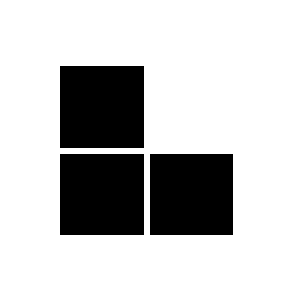
\epsfig{file=Abbildungen/triomino.eps, scale=0.7}
  \caption{Ein Triomino.}
  \label{fig:triomino.eps}
\end{figure}

\vspace*{0.2cm}
 
\noindent  
\textbf{Hinweis 1:}  Beim Beweis einer mathematischen Behauptung ist es manchmal einfacher, zun\"{a}chst  
ein  Ergebnis zu beweisen, was allgemeiner ist als die eigentlich zu beweisende Behauptung.  Das mag  
zwar kontraintuitiv erscheinen, weil Sie dann ja offensichtlich mehr beweisen m\"{u}ssen, aber dieses  
Beispiel soll Ihnen zeigen, dass es tats\"{a}chlich F\"{a}lle gibt, wo Sie das Problem am einfachsten durch  
Verallgemeinerung l\"{o}sen k\"{o}nnen.  
\vspace*{0.2cm}

\noindent
\textbf{Hinweis 2:}  Um diese Aufgabe l\"{o}sen zu k\"{o}nnen, m\"{u}ssen Sie kein Schachspieler sein.
F\"{u}r den Zweck der Aufgabe reicht es zu wissen, dass ein Schachbrett ein Quadrat der L\"{a}nge 8 ist (was immer
dabei die L\"{a}ngeneinheit ist), das in $8 \times 8$ Quadrate der L\"{a}nge 1 unterteilt ist.
\exend  

%%% local Variables: 
%%% Mode: latex
%%% TeX-master: "lineare-algebra"
%%% End: 
